\documentclass[12pt,a4paper]{article}

\usepackage[utf8]{inputenc}
\usepackage[T1]{fontenc}
\usepackage[brazil]{babel}
\usepackage{lmodern}
\usepackage[a4paper,margin=2.5cm]{geometry}
\usepackage{amsmath,amssymb}
\usepackage{graphicx}
\usepackage{booktabs}
\usepackage{float}
\usepackage{caption}
\usepackage{xcolor}
\usepackage{listings}
\usepackage[hidelinks]{hyperref}

\definecolor{codebg}{RGB}{248,248,248}
\definecolor{codecomment}{RGB}{0,110,0}
\definecolor{codekw}{RGB}{0,0,160}
\definecolor{codestr}{RGB}{160,40,40}

\lstset{
  language=Python,
  basicstyle=\ttfamily\footnotesize,
  backgroundcolor=\color{codebg},
  keywordstyle=\color{codekw}\bfseries,
  commentstyle=\color{codecomment}\itshape,
  stringstyle=\color{codestr},
  numbers=left,
  numberstyle=\tiny\color{gray},
  frame=single,
  breaklines=true,
  showstringspaces=false,
  tabsize=4,
  inputencoding=utf8,
  extendedchars=true,
  literate=
    {á}{{\'a}}1 {à}{{\`a}}1 {ã}{{\~a}}1 {â}{{\^a}}1
    {é}{{\'e}}1 {ê}{{\^e}}1 {í}{{\'i}}1
    {ó}{{\'o}}1 {õ}{{\~o}}1 {ô}{{\^o}}1
    {ú}{{\'u}}1 {ç}{{\c{c}}}1
    {Á}{{\'A}}1 {É}{{\'E}}1 {Í}{{\'I}}1 {Ó}{{\'O}}1 {Ú}{{\'U}}1 {Ç}{{\c{C}}}1
}

% Link do repositório do código
\newcommand{\repositorio}{\url{https://github.com/juliaPamplona/teia-laboratorios}}

\begin{document}

%=====================================================================
% Capa (página 1)
%=====================================================================
\begin{titlepage}
\centering

\includegraphics[width=0.35\textwidth]{figuras/logo_uepb.jpg}\\[1.5em]
{\large \textsc{Universidade Estadual da Paraíba}}\\[0.3em]
{\normalsize Disciplina: Tópicos Especiais em Inteligência Artificial}\\[0.3em]
{\normalsize Prof. Robson Pequeno de Sousa}

\vfill

{\LARGE \textbf{Classificador de Distância Mínima e Funções de Decisão aplicados à base Iris}}\\[1em]
{\large Relatório do Laboratório 01 --- Reconhecimento com base em decisão teórica}

\vfill

{\large Júlia Pamplona}

\vfill

{\large Setembro de 2026}
\end{titlepage}

%=====================================================================
% Resumo (página 2)
%=====================================================================
\begin{abstract}
Este relatório descreve a implementação, em Python e sem o uso de bibliotecas de aprendizado de máquina, de um sistema de reconhecimento supervisionado de padrões para a base de dados Iris, fundamentado na abordagem de reconhecimento por decisão teórica. Foram implementados (i) o classificador de distância mínima, (ii) o classificador pelo máximo das funções de decisão e (iii) as superfícies de decisão entre pares de classes. Os modelos com quatro atributos obtiveram 91,11\% de acurácia no conjunto de teste, com predições idênticas nos dois classificadores, o que confirma empiricamente a equivalência teórica entre eles. As retas de decisão construídas com os dois primeiros atributos (sépala) separam bem a classe \emph{setosa} das demais, mas apresentam desempenho limitado no par \emph{versicolor}~$\times$~\emph{virginica}, devido à sobreposição das nuvens de dados nesse subespaço.

\vspace{1em}
\noindent\textbf{Palavras-chave:} reconhecimento de padrões; classificador de distância mínima; funções de decisão; superfície de decisão; base Iris.
\end{abstract}
\thispagestyle{empty}
\newpage

%=====================================================================
% Sumário (página 3)
%=====================================================================
\tableofcontents
\thispagestyle{empty}
\newpage

%=====================================================================
\section{Introdução}
%=====================================================================

O reconhecimento de padrões supervisionado parte do pressuposto de que há um conjunto de treinamento com rótulos conhecidos e de que o classificador é projetado explorando essa informação \emph{a priori}. Entre as técnicas clássicas dessa categoria estão o classificador de distância mínima, o método da máxima verossimilhança e o método de Bayes. Este laboratório trata da primeira delas e de sua formulação equivalente por funções de decisão.

A abordagem por decisão teórica baseia-se em encontrar $W$ funções de decisão (ou funções discriminantes) $d_1(\mathbf{x}), \dots, d_W(\mathbf{x})$ tais que um padrão $\mathbf{x}$ pertence à classe $\omega_i$ se $d_i(\mathbf{x})$ tiver o maior valor numérico entre todas elas.

O objetivo do trabalho é aplicar esses conceitos à base Iris, cumprindo os seguintes requisitos:
\begin{enumerate}
  \item dividir a amostra em 70\% para treinamento e 30\% para teste (a validação fica para um momento posterior);
  \item plotar diagramas de dispersão com os dois primeiros atributos nos cenários \emph{setosa}~$\times$~\emph{versicolor}, \emph{setosa}~$\times$~\emph{virginica} e \emph{versicolor}~$\times$~\emph{virginica};
  \item definir, com os quatro atributos, (i) o classificador de distância mínima e (ii) o classificador de máximo das funções de decisão, ambos para as três classes;
  \item (iii) definir a superfície de decisão (reta) com os dois primeiros atributos para os três cenários e visualizá-la sobre o conjunto de teste e sobre toda a amostra;
  \item não utilizar bibliotecas de aprendizado de máquina.
\end{enumerate}

%=====================================================================
\section{Fundamentação teórica}\label{sec:teoria}
%=====================================================================

\subsection{Funções de decisão e fronteiras}

Seja $\mathbf{x} = [x_1, x_2, \dots, x_n]^t$ um vetor de características $n$-dimensional associado às classes $\omega_1, \omega_2, \dots, \omega_W$. A regra de decisão é
\begin{equation}
  \mathbf{x} \in \omega_i \quad \text{se} \quad d_i(\mathbf{x}) > d_j(\mathbf{x}), \quad j \neq i = 1, 2, \dots, W.
  \label{eq:regra}
\end{equation}

A fronteira de decisão que separa $\omega_i$ de $\omega_j$ é o lugar geométrico onde as duas funções se igualam:
\begin{equation}
  d_{ij}(\mathbf{x}) = d_i(\mathbf{x}) - d_j(\mathbf{x}) = 0,
  \label{eq:fronteira}
\end{equation}
de modo que $d_{ij}(\mathbf{x}) > 0 \Rightarrow \mathbf{x} \in \omega_i$ e $d_{ij}(\mathbf{x}) < 0 \Rightarrow \mathbf{x} \in \omega_j$.

\subsection{Reconhecimento baseado em casamento: classificador de distância mínima}

No reconhecimento baseado em casamento, cada classe é representada por um vetor protótipo, e um padrão desconhecido é atribuído à classe mais próxima segundo uma métrica predefinida. O caso mais simples é o classificador de distância mínima com distância euclidiana. O protótipo da classe $\omega_j$ é o vetor média de suas amostras:
\begin{equation}
  \mathbf{m}_j = \frac{1}{N_j} \sum_{\mathbf{x} \in \omega_j} \mathbf{x}, \qquad j = 1, 2, \dots, W,
  \label{eq:prototipo}
\end{equation}
onde $N_j$ é o número de vetores da classe $\omega_j$. A distância euclidiana ao protótipo é
\begin{equation}
  D_j(\mathbf{x}) = \lVert \mathbf{x} - \mathbf{m}_j \rVert = \sqrt{(\mathbf{x} - \mathbf{m}_j)^t (\mathbf{x} - \mathbf{m}_j)},
  \label{eq:distancia}
\end{equation}
e o padrão é associado à classe do protótipo mais próximo: $\mathbf{x} \in \omega_j$ se $D_j(\mathbf{x})$ for a menor entre todas as distâncias.

\subsection{Equivalência entre distância mínima e máximo da função de decisão}\label{sec:equivalencia}

Quando a distância é euclidiana, selecionar a menor distância equivale a determinar o máximo da função de decisão
\begin{equation}
  d_j(\mathbf{x}) = \mathbf{x}^t \mathbf{m}_j - \frac{1}{2} \mathbf{m}_j^t \mathbf{m}_j, \qquad j = 1, 2, \dots, W.
  \label{eq:decisao}
\end{equation}

A equivalência decorre de expandir o quadrado da distância:
\begin{equation}
  D_j^2(\mathbf{x}) = \mathbf{x}^t\mathbf{x} - 2\,\mathbf{x}^t\mathbf{m}_j + \mathbf{m}_j^t\mathbf{m}_j
  = \mathbf{x}^t\mathbf{x} - 2\left(\mathbf{x}^t \mathbf{m}_j - \tfrac{1}{2}\mathbf{m}_j^t \mathbf{m}_j\right)
  = \mathbf{x}^t\mathbf{x} - 2\, d_j(\mathbf{x}).
\end{equation}
Como $\mathbf{x}^t\mathbf{x}$ é o mesmo para todas as classes e a raiz quadrada é monotônica, minimizar $D_j$ é o mesmo que maximizar $d_j$. Portanto, os classificadores (i) e (ii) devem produzir \emph{exatamente} as mesmas predições, fato verificado experimentalmente na Seção~\ref{sec:resultados}.

\subsection{Superfície de decisão do classificador de distância mínima}

Substituindo a Eq.~\eqref{eq:decisao} na Eq.~\eqref{eq:fronteira}, obtém-se
\begin{equation}
  d_{ij}(\mathbf{x}) = (\mathbf{m}_i - \mathbf{m}_j)^t \mathbf{x} - \frac{1}{2}(\mathbf{m}_i - \mathbf{m}_j)^t(\mathbf{m}_i + \mathbf{m}_j) = 0.
  \label{eq:superficie}
\end{equation}
Essa superfície é o \emph{bissetor perpendicular} ao segmento que liga $\mathbf{m}_i$ e $\mathbf{m}_j$: o vetor normal ao hiperplano é $\mathbf{w} = \mathbf{m}_i - \mathbf{m}_j$ (portanto paralelo ao segmento), e o ponto médio $(\mathbf{m}_i + \mathbf{m}_j)/2$ satisfaz a equação. Com $n=2$ atributos a superfície é uma reta; com $n=4$, um hiperplano.

Escrevendo a Eq.~\eqref{eq:superficie} na forma $\mathbf{w}^t\mathbf{x} + w_0 = 0$, tem-se
\begin{equation}
  \mathbf{w} = \mathbf{m}_i - \mathbf{m}_j, \qquad
  w_0 = -\frac{1}{2}\left(\mathbf{m}_i^t\mathbf{m}_i - \mathbf{m}_j^t\mathbf{m}_j\right),
  \label{eq:coef}
\end{equation}
pois $(\mathbf{m}_i - \mathbf{m}_j)^t(\mathbf{m}_i + \mathbf{m}_j) = \mathbf{m}_i^t\mathbf{m}_i - \mathbf{m}_j^t\mathbf{m}_j$. Essa é a forma usada na implementação.

\subsection{Exemplo ilustrativo}

Um exemplo clássico do método é a separação entre \emph{Iris versicolor} ($\omega_1$) e \emph{Iris setosa} ($\omega_2$) usando comprimento e largura da pétala, com protótipos $\mathbf{m}_1 = (4{,}3;\ 1{,}3)^t$ e $\mathbf{m}_2 = (1{,}5;\ 0{,}3)^t$. A superfície resultante é $d_{12}(\mathbf{x}) = 2{,}8x_1 + 1{,}0x_2 - 8{,}9 = 0$, com a regra: $\mathbf{x} \in \omega_1$ se $d_{12}(\mathbf{x}) > 0$ e $\mathbf{x} \in \omega_2$ se $d_{12}(\mathbf{x}) < 0$. Pode-se conferir pela Eq.~\eqref{eq:coef}: $\mathbf{w} = (2{,}8;\ 1{,}0)^t$ e $w_0 = -\tfrac{1}{2}(20{,}18 - 2{,}34) = -8{,}92$. Este laboratório reproduz o mesmo procedimento, mas com os dois primeiros atributos da base (dimensões da \emph{sépala}), conforme exigido pelo enunciado, e o estende aos três pares de classes.

%=====================================================================
\section{Base de dados}
%=====================================================================

A base Iris (arquivo \texttt{Iris data.xls}) contém 150 amostras, 50 de cada espécie: \emph{setosa}, \emph{versicolor} e \emph{virginica}. Cada amostra é descrita por quatro atributos, que formam o vetor de características $\mathbf{x} = [x_1, x_2, x_3, x_4]^t$. A ordem das colunas no arquivo, e portanto a adotada neste trabalho, é:

\begin{table}[H]
\centering
\caption{Atributos da base Iris na ordem do arquivo.}
\begin{tabular}{cll}
\toprule
Atributo & Coluna & Descrição \\
\midrule
$x_1$ & \texttt{Sepal length} & comprimento da sépala (cm) \\
$x_2$ & \texttt{Sepal width}  & largura da sépala (cm) \\
$x_3$ & \texttt{Petal length} & comprimento da pétala (cm) \\
$x_4$ & \texttt{Petal width}  & largura da pétala (cm) \\
\bottomrule
\end{tabular}
\end{table}

Assim, os ``dois primeiros atributos'' pedidos no enunciado correspondem, aqui, às dimensões da sépala, e não às da pétala usadas no exemplo ilustrativo.

%=====================================================================
\section{Metodologia e implementação}
%=====================================================================

O código foi escrito em Python~3.12 usando apenas \texttt{pandas} (leitura da planilha e manipulação tabular), \texttt{numpy} (álgebra vetorial) e \texttt{matplotlib} (gráficos). Nenhuma biblioteca de aprendizado de máquina foi utilizada: médias, distâncias, funções de decisão, superfícies, divisão da amostra, matriz de confusão e acurácia foram implementadas manualmente. O código-fonte completo, a base de dados e as figuras geradas estão disponíveis no repositório \repositorio. Os trechos apresentados a seguir mantêm a numeração de linhas do arquivo \texttt{lab01.py}.

\subsection{Divisão 70\% / 30\% estratificada}

Como o classificador é supervisionado, os protótipos precisam ser estimados apenas com dados de treinamento, e o desempenho deve ser medido em amostras não vistas. A divisão foi feita \emph{por classe}: as 50 amostras de cada espécie são embaralhadas e separadas em 35 para treino e 15 para teste, totalizando 105 e 45 amostras. A estratificação preserva a proporção de 1/3 por classe nos dois conjuntos. Uma versão preliminar que embaralhava a base inteira produziu um teste desbalanceado (10 \emph{setosa}, 17 \emph{versicolor}, 18 \emph{virginica}), o que motivou a correção. A semente aleatória é fixada (\texttt{np.random.seed(42)}) para reprodutibilidade.

\begin{lstlisting}[firstnumber=16]
np.random.seed(42)
train_idx, test_idx = [], []
for c in classes:
    idx_c = np.random.permutation(np.where(df[target] == c)[0])
    n_train = int(round(0.7 * len(idx_c)))
    train_idx.extend(idx_c[:n_train])
    test_idx.extend(idx_c[n_train:])
\end{lstlisting}

\subsection{Vetores protótipos}

Os protótipos são as médias por classe do conjunto de treino, exatamente como na Eq.~\eqref{eq:prototipo}. São calculados dois conjuntos: \texttt{means\_4d}, com os quatro atributos, usado nos classificadores (i) e (ii); e \texttt{means\_2d}, com os dois primeiros, usado nas retas do item (iii).

\begin{lstlisting}[firstnumber=32]
means_4d = {c: train_data[train_data[target] == c][atributos_4d].mean().values for c in classes}
means_2d = {c: train_data[train_data[target] == c][atributos_2d].mean().values for c in classes}
\end{lstlisting}

\subsection{(i) Classificador de distância mínima}

A função \texttt{dist\_euclidiana} implementa a Eq.~\eqref{eq:distancia}. Para cada amostra de teste calcula-se a distância aos três protótipos e escolhe-se a classe de menor distância:

\begin{lstlisting}[firstnumber=41]
def dist_euclidiana(x, m):
    return np.sqrt(np.sum((x - m)**2))
\end{lstlisting}

\subsection{(ii) Classificador pelo máximo das funções de decisão}

A função \texttt{func\_decisao} implementa a Eq.~\eqref{eq:decisao}, e a classe atribuída é a de maior $d_j(\mathbf{x})$, segundo a regra da Eq.~\eqref{eq:regra}. O programa também imprime cada função de decisão de forma explícita, com os coeficientes numéricos, para que o modelo possa ser inspecionado:

\begin{lstlisting}[firstnumber=49]
def func_decisao(x, m):
    return np.dot(x, m) - 0.5 * np.dot(m, m)
\end{lstlisting}

O laço de avaliação aplica os dois classificadores a cada amostra de teste. Além da acurácia, o programa verifica se as listas de predições coincidem e monta uma matriz de confusão implementada manualmente.

\subsection{(iii) Superfícies de decisão}

A função \texttt{coef\_superficie} retorna $\mathbf{w}$ e $w_0$ conforme a Eq.~\eqref{eq:coef}, equivalente à Eq.~\eqref{eq:superficie}. A mesma função atende ao caso 4D (hiperplanos) e ao caso 2D (retas). A função \texttt{classifica\_par} aplica a regra de sinal associada à Eq.~\eqref{eq:fronteira}, ou seja, $d_{ij}(\mathbf{x}) > 0 \Rightarrow \omega_i$ e $d_{ij}(\mathbf{x}) < 0 \Rightarrow \omega_j$, o que permite medir quantas amostras cada reta separa corretamente:

\begin{lstlisting}[firstnumber=85]
def coef_superficie(mi, mj):
    w = mi - mj
    w0 = -0.5 * (np.dot(mi, mi) - np.dot(mj, mj))
    return w, w0

# Regra de decisão: d_ij(x) > 0 -> w_i ; d_ij(x) < 0 -> w_j
def classifica_par(X, w, w0, ci, cj):
    return np.where(X @ w + w0 > 0, ci, cj)
\end{lstlisting}

\subsection{Visualização}

Foram geradas três figuras, cada uma com os três cenários pedidos:
\begin{itemize}
  \item \textbf{Variabilidade}: dispersão de todas as 100 amostras do par, sem reta, para observar a nuvem de dados;
  \item \textbf{Teste}: apenas as amostras de teste do par, com a reta de decisão;
  \item \textbf{Dataset completo}: todas as amostras do par, com a mesma reta.
\end{itemize}
Nas figuras com reta, a função \texttt{plot\_reta} também marca os protótipos $\mathbf{m}_i$ e $\mathbf{m}_j$ (símbolo $\times$) e o segmento que os liga, evidenciando a construção geométrica da superfície de decisão. Os eixos usam a mesma escala (\texttt{set\_aspect('equal')}), para que a perpendicularidade entre a reta e o segmento $\overline{\mathbf{m}_i\mathbf{m}_j}$, prevista pela Eq.~\eqref{eq:superficie}, fique visível. Os limites dos eixos são fixados antes de desenhar a reta, de modo que ela não expanda a escala e ``achate'' a nuvem de pontos.

A reta é desenhada isolando $x_2$ em $w_1x_1 + w_2x_2 + w_0 = 0$, isto é, $x_2 = -(w_1x_1 + w_0)/w_2$. Há tratamento para o caso degenerado $w_2 = 0$ (reta vertical).

%=====================================================================
\section{Resultados}\label{sec:resultados}
%=====================================================================

\subsection{Protótipos e funções de decisão (4 atributos)}

\begin{table}[H]
\centering
\caption{Vetores protótipos $\mathbf{m}_j$ estimados no conjunto de treino (35 amostras por classe).}
\label{tab:prototipos}
\begin{tabular}{lcccc}
\toprule
Classe & $x_1$ & $x_2$ & $x_3$ & $x_4$ \\
\midrule
\emph{setosa}     & 4,989 & 3,426 & 1,486 & 0,240 \\
\emph{versicolor} & 5,949 & 2,731 & 4,237 & 1,309 \\
\emph{virginica}  & 6,683 & 3,009 & 5,631 & 2,069 \\
\bottomrule
\end{tabular}
\end{table}

Substituindo os protótipos na Eq.~\eqref{eq:decisao}, obtêm-se as funções de decisão:
\begin{align*}
d_{\text{setosa}}(\mathbf{x})     &= 4{,}989x_1 + 3{,}426x_2 + 1{,}486x_3 + 0{,}240x_4 - 19{,}443\\
d_{\text{versicolor}}(\mathbf{x}) &= 5{,}949x_1 + 2{,}731x_2 + 4{,}237x_3 + 1{,}309x_4 - 31{,}256\\
d_{\text{virginica}}(\mathbf{x})  &= 6{,}683x_1 + 3{,}009x_2 + 5{,}631x_3 + 2{,}069x_4 - 44{,}852
\end{align*}

\subsection{Desempenho dos classificadores (i) e (ii)}

Os dois classificadores obtiveram \textbf{91,11\%} de acurácia (41 acertos em 45) no conjunto de teste, e o programa confirmou que as 45 predições são idênticas. Esse é o resultado previsto pela equivalência demonstrada na Seção~\ref{sec:equivalencia}: não há erro de implementação no fato de as acurácias coincidirem, pois se trata do mesmo classificador escrito de duas formas.

\begin{table}[H]
\centering
\caption{Matriz de confusão no conjunto de teste (idêntica para os classificadores (i) e (ii)).}
\label{tab:confusao}
\begin{tabular}{lccc}
\toprule
Real $\backslash$ Predita & \emph{setosa} & \emph{versicolor} & \emph{virginica} \\
\midrule
\emph{setosa}     & \textbf{15} & 0 & 0 \\
\emph{versicolor} & 0 & \textbf{14} & 1 \\
\emph{virginica}  & 0 & 3 & \textbf{12} \\
\bottomrule
\end{tabular}
\end{table}

A classe \emph{setosa} é reconhecida sem erros. Todos os quatro erros ocorrem entre \emph{versicolor} e \emph{virginica}, classes cujos protótipos são mais próximos entre si (Tabela~\ref{tab:prototipos}).

\subsection{Superfícies de decisão com 4 atributos}\label{sec:hiperplanos}

Aplicando a Eq.~\eqref{eq:superficie} aos protótipos 4D, obtêm-se os hiperplanos:
\begin{align*}
\textit{setosa} \times \textit{versicolor}:&\quad -0{,}96x_1 + 0{,}69x_2 - 2{,}75x_3 - 1{,}07x_4 + 11{,}81 = 0\\
\textit{setosa} \times \textit{virginica}:&\quad -1{,}69x_1 + 0{,}42x_2 - 4{,}15x_3 - 1{,}83x_4 + 25{,}41 = 0\\
\textit{versicolor} \times \textit{virginica}:&\quad -0{,}73x_1 - 0{,}28x_2 - 1{,}39x_3 - 0{,}76x_4 + 13{,}60 = 0
\end{align*}
Os maiores coeficientes em módulo estão em $x_3$ e $x_4$ (pétala), indicando que é nessas direções que os protótipos mais se afastam. Isso é coerente com o uso dos atributos da pétala no exemplo ilustrativo.

\subsection{Diagramas de dispersão: variabilidade}

\begin{figure}[H]
\centering
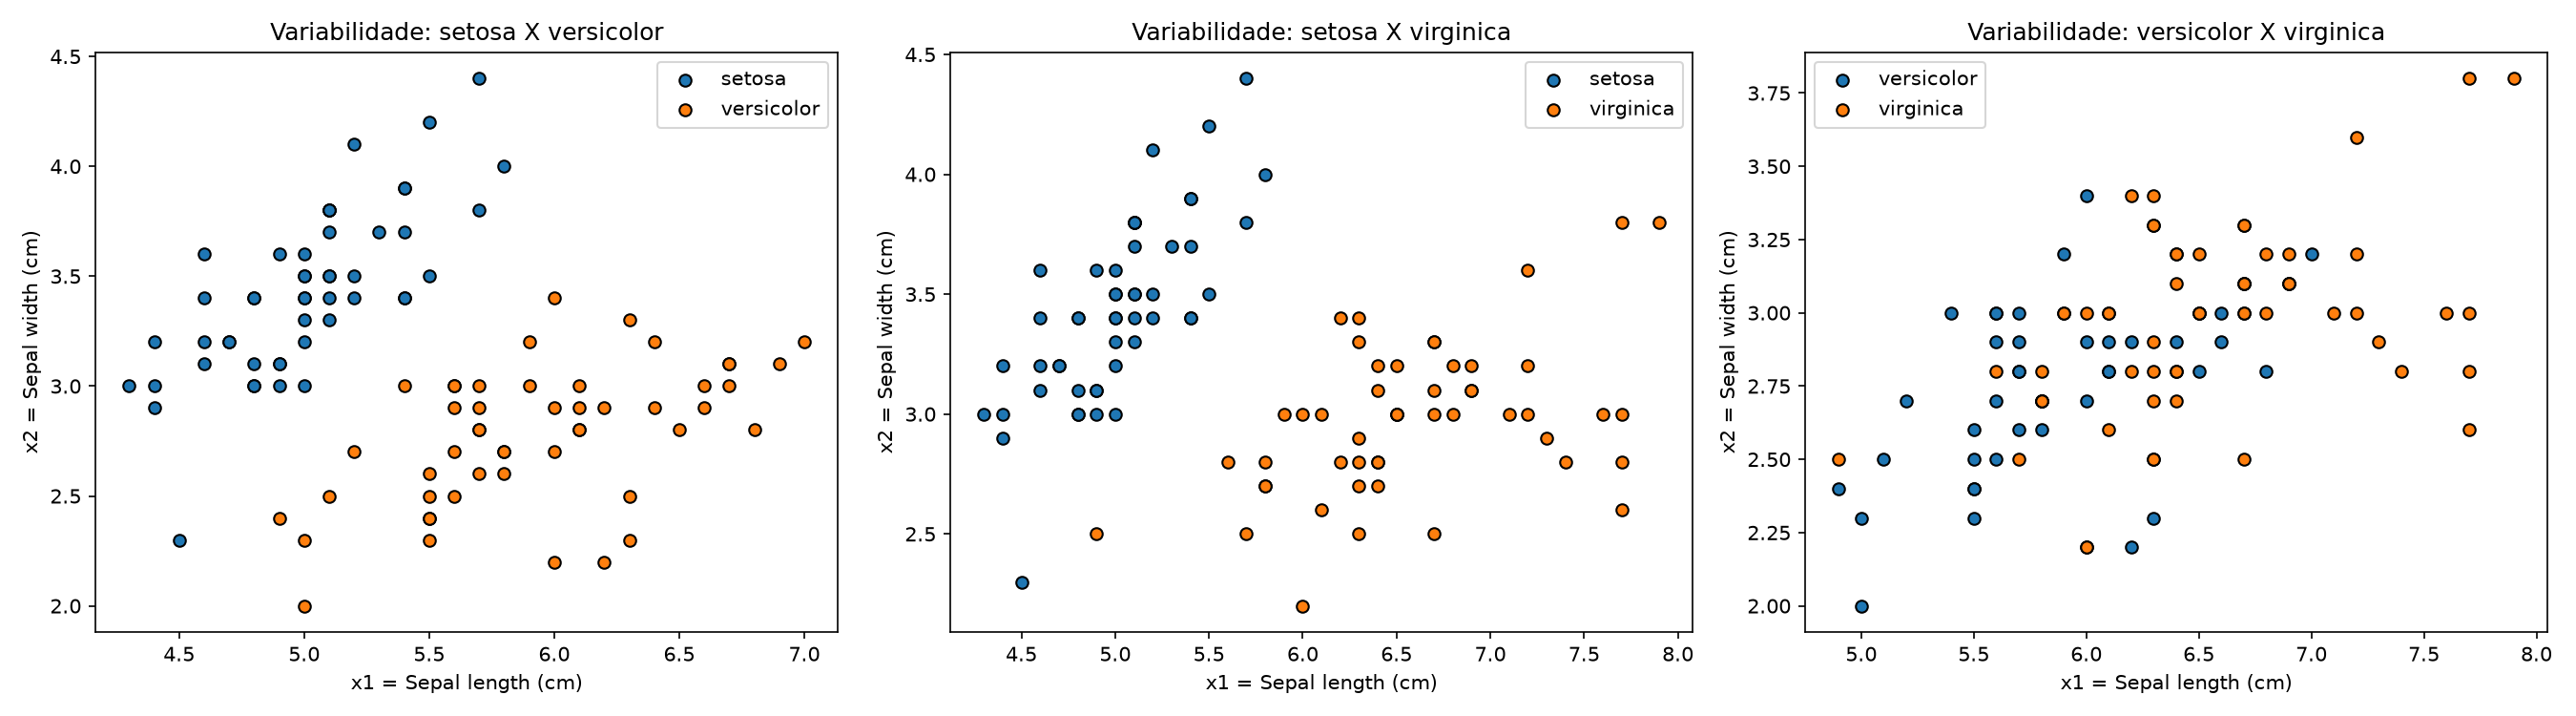
\includegraphics[width=\textwidth]{figuras/variabilidade.png}
\caption{Dispersão das 100 amostras de cada par usando os dois primeiros atributos (sépala).}
\label{fig:variabilidade}
\end{figure}

A Figura~\ref{fig:variabilidade} mostra que a nuvem de \emph{setosa} é compacta e deslocada para comprimentos menores e larguras maiores de sépala, afastada das demais. Já \emph{versicolor} e \emph{virginica} ocupam regiões muito sobrepostas, diferenciando-se apenas por uma tendência de \emph{virginica} a ter sépalas mais longas.

\subsection{Retas de decisão (2 atributos)}

Aplicando a Eq.~\eqref{eq:superficie} aos protótipos restritos a $(x_1, x_2)$, obtêm-se as retas da Tabela~\ref{tab:retas}. A acurácia foi medida pela regra de sinal de $d_{ij}(\mathbf{x})$.

\begin{table}[H]
\centering
\caption{Retas de decisão $d_{ij}(\mathbf{x}) = 0$ e acurácia da regra $d_{ij}(\mathbf{x}) \gtrless 0$.}
\label{tab:retas}
\begin{tabular}{llcc}
\toprule
Cenário ($\omega_i \times \omega_j$) & Reta de decisão & Teste & Completo \\
\midrule
\emph{setosa} $\times$ \emph{versicolor}    & $-0{,}96x_1 + 0{,}69x_2 + 3{,}11 = 0$ & 28/30 (93,3\%) & 98/100 (98\%) \\
\emph{setosa} $\times$ \emph{virginica}     & $-1{,}69x_1 + 0{,}42x_2 + 8{,}55 = 0$ & 29/30 (96,7\%) & 98/100 (98\%) \\
\emph{versicolor} $\times$ \emph{virginica} & $-0{,}73x_1 - 0{,}28x_2 + 5{,}43 = 0$ & 20/30 (66,7\%) & 72/100 (72\%) \\
\bottomrule
\end{tabular}
\end{table}

Como verificação, no par \emph{setosa} $\times$ \emph{versicolor} tem-se $\mathbf{w} = \mathbf{m}_{\text{set}} - \mathbf{m}_{\text{vers}} = (4{,}989 - 5{,}949;\ 3{,}426 - 2{,}731)^t = (-0{,}96;\ 0{,}69)^t$ e
$w_0 = -\tfrac{1}{2}(36{,}63 - 42{,}85) = 3{,}11$, conforme a Eq.~\eqref{eq:coef}.

\begin{figure}[H]
\centering
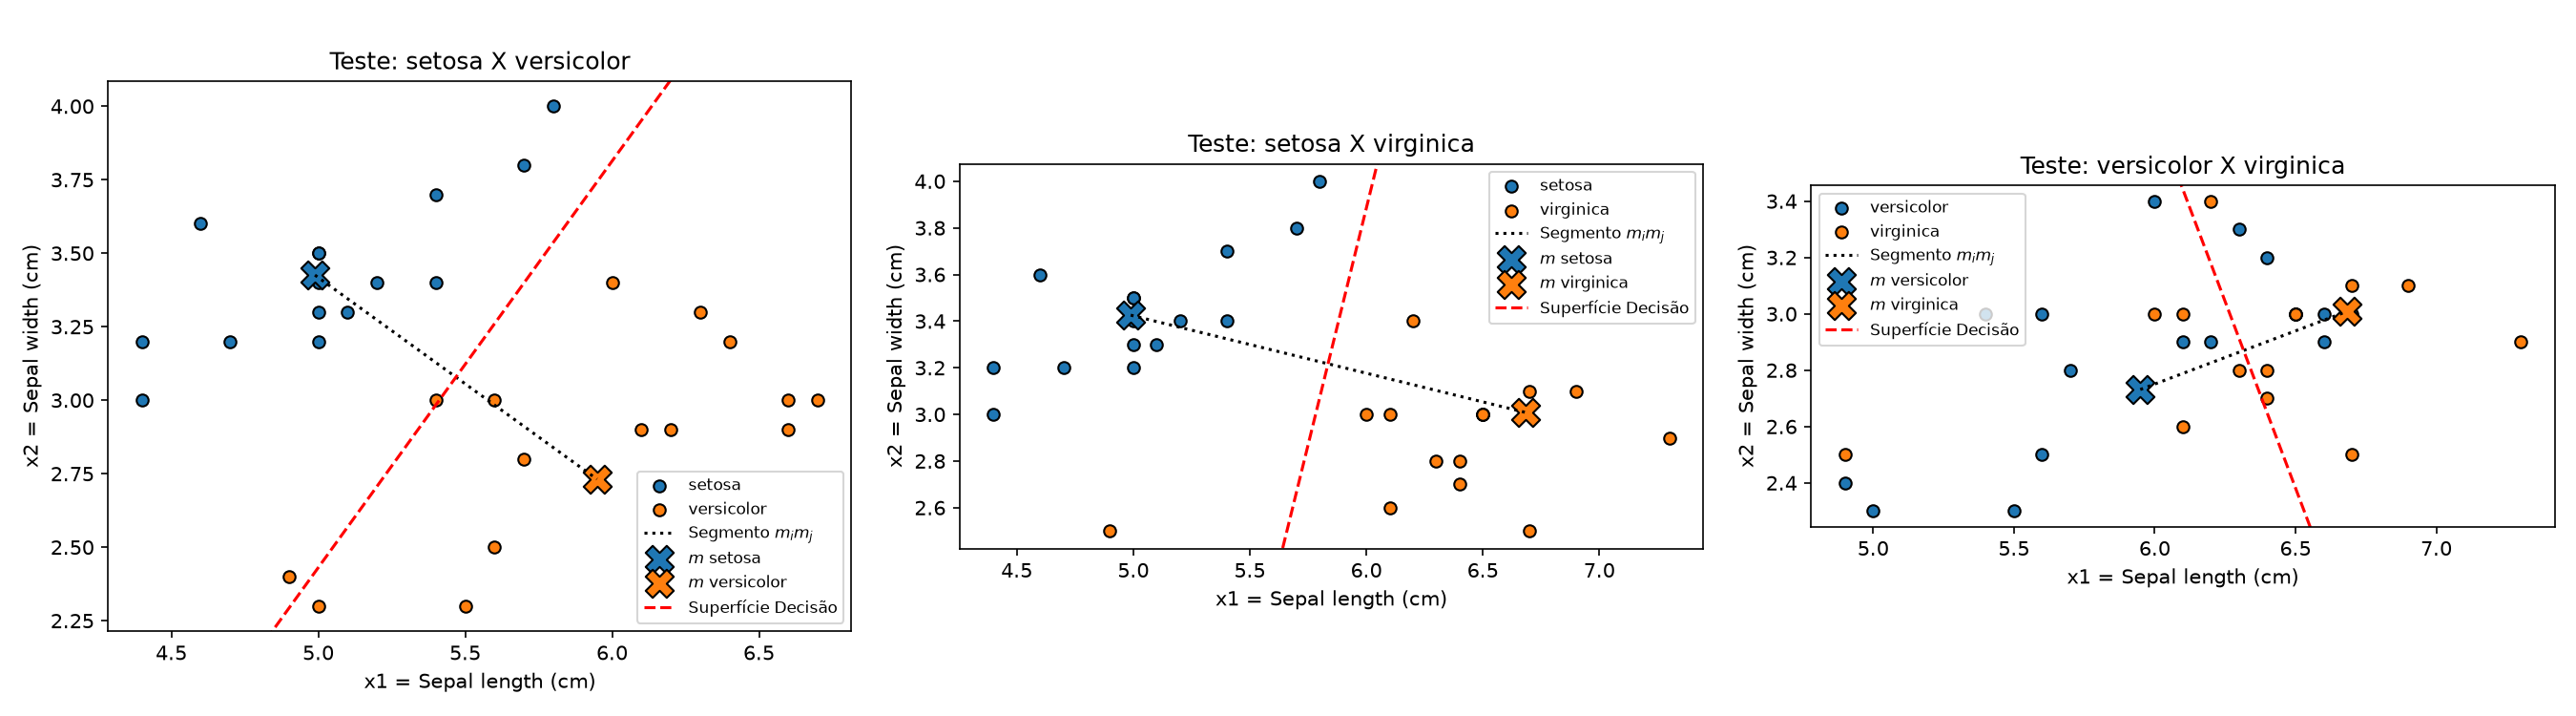
\includegraphics[width=\textwidth]{figuras/superficie_teste.png}
\caption{Retas de decisão sobre as amostras do conjunto de teste. Os símbolos $\times$ marcam os protótipos, e a linha pontilhada, o segmento $\overline{\mathbf{m}_i\mathbf{m}_j}$.}
\label{fig:teste}
\end{figure}

\begin{figure}[H]
\centering
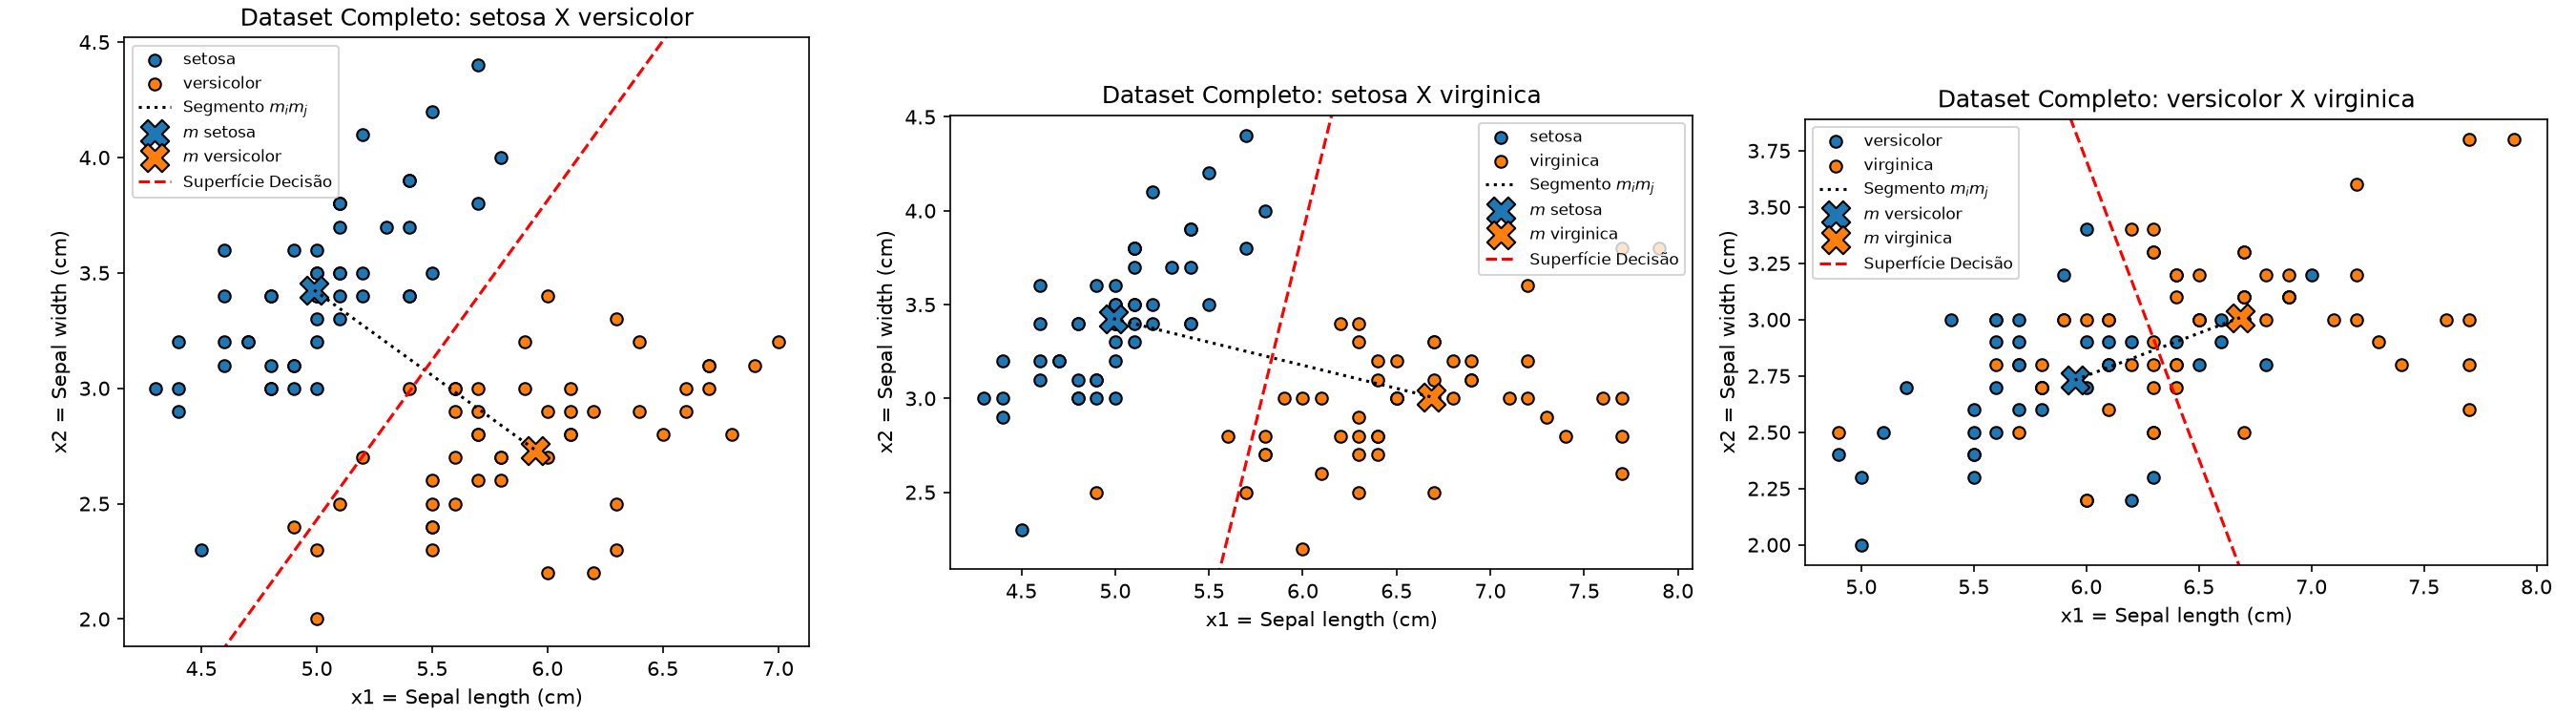
\includegraphics[width=\textwidth]{figuras/superficie_completo.png}
\caption{As mesmas retas, estimadas apenas com o treino, sobre todas as amostras de cada par.}
\label{fig:completo}
\end{figure}

As Figuras~\ref{fig:teste} e~\ref{fig:completo} evidenciam a propriedade geométrica da superfície de decisão do classificador de distância mínima: em todos os cenários a reta tracejada cruza o segmento $\overline{\mathbf{m}_i\mathbf{m}_j}$ no ponto médio e perpendicularmente a ele.

%=====================================================================
\section{Discussão}
%=====================================================================

\paragraph{Equivalência (i) $\equiv$ (ii).} As acurácias e predições idênticas confirmam, na prática, que selecionar a menor distância euclidiana equivale a determinar o máximo da função de decisão. A vantagem da forma (ii) é computacional e conceitual: $d_j(\mathbf{x})$ é \emph{linear} em $\mathbf{x}$ e dispensa a raiz quadrada. Por isso as fronteiras entre classes são hiperplanos, o que permite escrevê-las explicitamente, como na Seção~\ref{sec:hiperplanos}.

\paragraph{Separabilidade e escolha de atributos.} Com os quatro atributos o classificador atinge 91,11\%. Com apenas as dimensões da sépala, as retas que envolvem \emph{setosa} separam quase perfeitamente as classes (98\% na amostra completa), mas o par \emph{versicolor} $\times$ \emph{virginica} fica em 72\%. A causa é visível na Figura~\ref{fig:variabilidade}: nesse subespaço as nuvens se sobrepõem, e nenhuma reta, seja qual for o método, consegue separá-las bem. No exemplo ilustrativo são usadas as dimensões da pétala, em que as classes são muito mais separáveis, o que também se reflete nos coeficientes dominantes em $x_3$ e $x_4$ dos hiperplanos 4D.

\paragraph{Limitações do método.} O classificador de distância mínima representa cada classe apenas pela média, ignorando a dispersão e a correlação entre atributos. Ele funciona bem quando as classes formam nuvens aproximadamente esféricas, de tamanhos semelhantes e bem afastadas. Nos demais casos, métodos que modelam a variabilidade, como a máxima verossimilhança e o classificador de Bayes, tendem a ser mais adequados. Além disso, a distância euclidiana é sensível à escala dos atributos; na Iris todos estão em centímetros e em faixas comparáveis, o que atenua o problema.

\paragraph{Avaliação.} Os resultados vêm de uma única partição 70/30 com semente fixa, e o conjunto de teste tem apenas 45 amostras: cada erro equivale a cerca de 2,2 pontos percentuais. Uma estimativa mais robusta exigiria validação (por exemplo, validação cruzada), que, conforme o enunciado, ficará para um momento posterior.

%=====================================================================
\section{Conclusão}
%=====================================================================

Foram implementados, sem bibliotecas de aprendizado de máquina, o classificador de distância mínima, o classificador pelo máximo das funções de decisão e as superfícies de decisão entre pares de classes, seguindo fielmente a formulação do reconhecimento por decisão teórica. Os resultados reproduziram as propriedades teóricas do método: (a) os dois classificadores são equivalentes e produziram as mesmas predições, com 91,11\% de acurácia no teste; (b) as superfícies de decisão são bissetores perpendiculares ao segmento entre os protótipos, o que pode ser observado nos gráficos; e (c) a qualidade da separação depende fortemente dos atributos escolhidos, já que a sépala separa bem a \emph{setosa} mas não distingue \emph{versicolor} de \emph{virginica}, ao contrário da pétala.

%=====================================================================
% Referências
%=====================================================================
\begin{thebibliography}{9}

\bibitem{sousa}
SOUSA, R. P. de. \textbf{Reconhecimento: base em decisão teórica}. Material de aula da disciplina Tópicos Especiais em Inteligência Artificial. Campina Grande: Universidade Estadual da Paraíba, 2026.

\bibitem{repo}
PAMPLONA, J. \textbf{Laboratório 01: classificador de distância mínima e funções de decisão aplicados à base Iris}. Repositório de código-fonte, 2026. Disponível em: \repositorio. Acesso em: set. 2026.

\end{thebibliography}

\end{document}
